\documentclass[a4paper,11pt]{article}
\usepackage[english, czech]{babel}
\usepackage[utf8]{inputenc}
\usepackage[IL2]{fontenc}
\usepackage{times}
\usepackage{graphics}
\usepackage{tabularx}
\usepackage{multicol}
\usepackage{multirow}
\usepackage{pdflscape}
\usepackage{enumitem}
\usepackage{natbib}
\usepackage{url}
\usepackage{graphicx}
\usepackage{amsfonts}
\usepackage{float}
\usepackage[table,xcdraw]{xcolor}

\usepackage[total={16cm, 23cm}]{geometry}
\usepackage{mathtools}


\begin{document}
\begin{titlepage}
\begin{center}
\Huge
\textsc{Fakulta informačních technologií\\
Vysoké učení technické v Brně}\\
\vspace{\stretch{0.4}}
		\begin{figure}[ht]
		    
			\centering
			\scalebox{1}{\includegraphics[width=0.7\linewidth]{images/fit_logo.png}}
		\end{figure}
\vspace{\stretch{0.618}}
\LARGE Projektová praxe (IPP) \\\
Technická zpráva k projektu Morphing otisků prstů\\
\vspace{\stretch{0.8}}
\Large Květen 2020 \hfill Daniel Kolínek (xkolin05) \newpage
\end{center}
\end{titlepage}

\newpage
\begin{multicols*}{2}
\section{Abstrakt}
    Cílem práce bylo implementovat aplikaci, která umožňuje generování otisků ze dvou zadaných. Takový otisk poté může obsahovat dostatečné informace z obou otisků prstů, aby seděl na oba zároveň.

\section{Úvod}
    Na morphingu obrazu se pracovalo již v 80. letech minulého století, kdy v roce 1989 filmový průmysl byla použita technika mesh warping technique ve filmu Indiana Jones and the Last Crusade. A proto není divu, že v posledních letech, kdy se používají pro zabezpečení biometrické údaje jako je otisk prstu nebo obličej, dochází k morfologickým útokům. Nebezpečná je tato technika z toho důvodu, že dvě osoby po morphingu svých biometrických údajů mohou při správném morfování dosáhnout toho, že oba mohou použít např. jeden doklad totožnosti, či přístupovou kartu. 

\section{Předzpracování otisků} 
    Otisk prstu je stopa, kterou zanechávají papilární linie. Na běžném snímku otisku je papilární linie zaznamenána pomocí černé barvy (stupně šedi) a údolí mezi nimi pomocí bílé barvy, s čímž počítá i má implementace.
    
    Pro co nejreálnější výsledky morphingu je zapotřebí, před jeho provedením, zajistit, aby si otisky byly co nejvíce podobné. Prvně se tedy obrázky otisků normalizují pomocí funkce OpenCV cv2.normalize. Po normalizaci je provedeno oříznutí pozadí. 
    
    \subsection{Zarovnání otisků}
        Pro najití nejlepší pozice zarovnání dvou otisků prstů byla použita technika pracující na úrovni orientovaných polí. Hlavně z toho důvodu, že dva odlišné otisky mohou mít úplně jiné rysy, jako například jeden může obsahovat core point, druhý ne. O tom píši v kapitole \ref{miniatue}. Nejprve tedy něco k orientovanému poli.

        \subsubsection{Orientované pole}
        Nechť [x, y] je bod (pixel) v obrazu otisku. Pak lokální orientace linie v bodě [x, y] je úhel $\theta_{x,y}$, který svírají linie, procházející skrz libovolně velké okolí se středem v bodě [x, y], s vodorovnou osou. Protože hřebeny otisku jsou nesměrové, $\theta_{x,y}$ je neorientovaný směr v rozmezí [0..$\pi$]. Orientované pole je poté matice D, v jejíž prvcích je uložena lokální orientace linií v daném okolí. Každý prvek $\theta_{x,y}$ matice D udává průměrnou orientaci linií v okolí bodu [x, y], kde bod [x, y] reprezentuje čtvercovou mřížku umístěnou nad tímto bodem viz. obrázek \ref{fig:ori}. S každým prvkem $\theta_{x,y}$ je často asociována hodnota $r_{x,y}$, která označuje míru spolehlivosti orientace.
        
        \begin{figure}[H]
            \centering
                {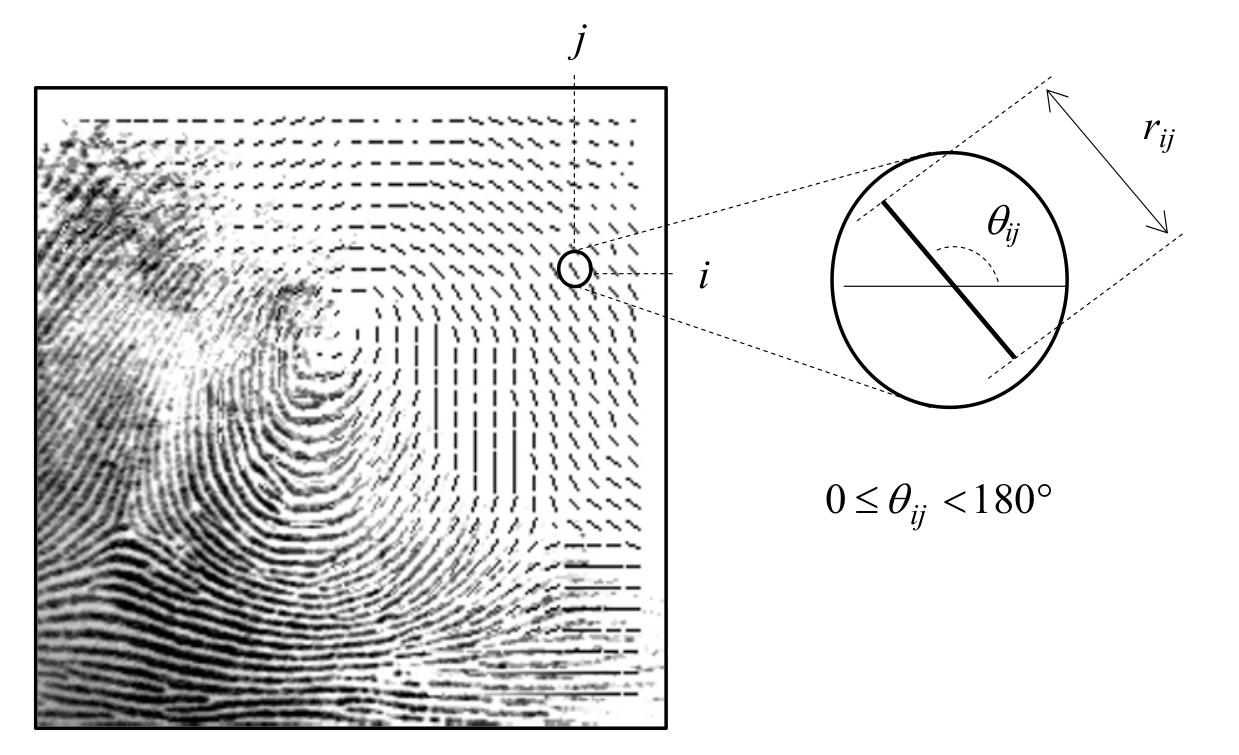
\includegraphics[width=0.8\linewidth]{images/ori.png}}\\
                \caption{Vlevo původní obraz otisku, vpravo orientované pole}
                \label{fig:ori}
        \end{figure}
        
        Popis algoritmu:
        \begin{enumerate}
            \item Rozdělíme normalizovaný obraz $\mathcal{G}$ na bloky o velikosti w*w. V aktuální implementaci pokud se na celém bloku nevyskytuje žádná linie, poté je ihned označena hodnota bloku za 0 a r nastaveno na 0, v opačném případě se r nastaví na 1 a pokračuje se ve výpočtu.
            
            \item Vypočítáme gradienty $\partial_{x}(i, j)$ a $\partial_{y}(i, j)$ pro každý pixel (i,j) pomocí Sobelova operátoru.
            \item Stanovíme lokální orientaci pro každý blok se středem v pixelu (i,j), pomocí následujících rovnic:
                \begin{equation} 
                    \mathcal{V}_{x}(i, j)=\sum_{u=i-\frac{w}{2}}^{i+\frac{w}{2}} \sum_{v=j-\frac{w}{2}}^{j+\frac{w}{2}} 2 \partial_{x}(u, v) \partial_{y}(u, v)
                \end{equation}
                \begin{equation} 
                    \begin{multlined}
                        \mathcal{V}_{y}(i, j)=\\\sum_{u=i-\frac{w}{2}}^{i+\frac{w}{2}} \sum_{v=j-\frac{w}{2}}^{j+\frac{w}{2}}\left(\partial_{x}^{2}(u, v)-\partial_{y}^{2}(u, v)\right)
                    \end{multlined}
                \end{equation}
                \begin{equation} 
                    \theta(i, j)=\frac{1}{2} \tan ^{-1}\left(\frac{\mathcal{V}_{y}(i, j)}{\mathcal{V}_{x}(i, j)}\right)
                \end{equation}
                 Kde $\theta(i, j)$ je nejmenší čtvercový odhad lokální orientace linií v bloku se středem v (i,j).
             \item Z důvodu výskytu šumu, nepravých linií, atp. nemusí vždy být lokální orientace $\theta(i, j)$ stanovena správně. Díky tomu, že se lokální orientace ve svém okolí mění pouze mírně, kde se neobjevují žádné singulární body, je pro opravu (vyhlazení) použit filtr s dolní propustí. Pro provedení operace filtrem je zapotřebí převést $\theta$ do vektorového pole, které je definováno následovně:
             \begin{equation}
                 \Phi_{x}(i, j)=\cos (2 \theta(i, j))
            \end{equation}   
            \begin{equation}
                 \Phi_{y}(i, j)=\sin (2 \theta(i, j))
             \end{equation}
             Následné filtrování filtrem s dolní propustí je provedeno:
             \begin{equation}
                 \begin{multlined}
                     \Phi_{x}^{\prime}(i, j)= \sum_{u=-w_{\Phi} / 2}^{w_{\Phi} / 2} \sum_{v=-w_{\Phi} / 2}^{w_{\Phi} / 2} \\ W(u, v) \Phi_{x}(i-u w, j-v w)
                \end{multlined}
             \end{equation}
             \begin{equation}
                \begin{multlined}
                     \Phi_{y}^{\prime}(i, j)=\sum_{u=-w_{\Phi} / 2}^{w_{\Phi} / 2} \sum_{v=-w_{\Phi} / 2}^{w_{\Phi} / 2} \\ W(u, v) \Phi_{y}(i-u w, j-v w)
                \end{multlined}
             \end{equation}
             Kde W je 2D filtr pro dolní propust. Defaultní velikost filtru je 5x5
             \item Výpočet vyhlazené lokální orientace se následně provádí pomocí:
              \begin{equation}
                \mathcal{O}(i, j)=\frac{1}{2} \tan \left(\frac{\Phi_{y}^{\prime}(i, j)}{\Phi_{x}^{\prime}(i, j)}\right)
             \end{equation}
        \end{enumerate}\cite{ori}
    
    Po stanovení orientovaného pole obou otisků prstů je konečně možné se pustit do jejich zarovnání. Metoda se snaží maximalizovat podobnost orientovaných polí v jejich průsečících.
    
    Orientovaná pole $\mathcal{O}_1$ a $\mathcal{O}_2$ jsou vypočítána po blocích  w x w a na každé pozici (i,j) obsahuje hodnotu velikosti úhlu $\theta$ a r = [0,1]. Poté je podobnost mezi orientovanými poly vypočítána:
    \begin{equation}
        \begin{multlined}
        S\left(\mathcal{O}^{1}, \mathcal{O}^{2}\right)=\\
        \frac{\sum_{(i, j) \in\left(V_{\mathcal{O} 1} \cap V_{\mathcal{O} 2}\right)}\left(r_{i, j}^{1}+r_{i, j}^{2}\right) \cdot \psi\left(\theta_{i, j}^{1}, \theta_{i, j}^{2}\right)}{\sum_{(i, j) \in\left(V_{\mathcal{O}^{1}} \cap V_{\mathcal{O}^{2}}\right)}\left(r_{i, j}^{1}+r_{i, j}^{2}\right)}
        \end{multlined}
    \end{equation}
    
    , kde $\psi\left(\theta_{1}, \theta_{2}\right) $ je podobnost dvou úhlů z orientovaných polí:
    \begin{equation}
        \psi\left(\theta_{1}, \theta_{2}\right)=1-\frac{2 \cdot\left|\theta_{1}-\theta_{2}\right|}{\pi}
    \end{equation}
    
    a $V_{\mathcal{O}}$ obsahuje pouze souřadnice z popředí:
    \begin{equation}
        V_{\mathcal{O}}=\left\{(i, j) | o_{i, j} \in \mathcal{O} \wedge r_{i, j}>0\right\}
    \end{equation}
    
    Následně pro optimalizaci se přeskakují pozice, dvou orientovaných polí, na kterých se dostatečně nepřekrývají.
    
    \begin{equation}
        \frac{\left|V_{\mathcal{O}^{1}} \cap V_{\mathcal{O}}\right|}{\max \left(\left|V_{\mathcal{O}^{1} }\right|, | V_{\mathcal{O}^{2} }|\right)} \geq min_{V R}
    \end{equation}
    
    V mé implementaci uvažuji pouze natočení v rozsahu $<-45^{\circ};45^{\circ}>$ a posun o maximálně 50\% šířky při posunu vpravo nebo vlevo a 50\% výšky při posunu nahoru, nebo dolu. Větší změny vedly buď k nepřesnostem, nebo neměly dopad na výsledek. Dále se snažím pokaždé nasadit menší otisk prstu na větší. Po zarovnání otisků se provede oříznutí částí, které nejsou jejich průnikem.
    
    Příklad výsledku je vidět na obrátku \ref{fig:prunik}.
    \begin{figure}[H]
        \centering
            {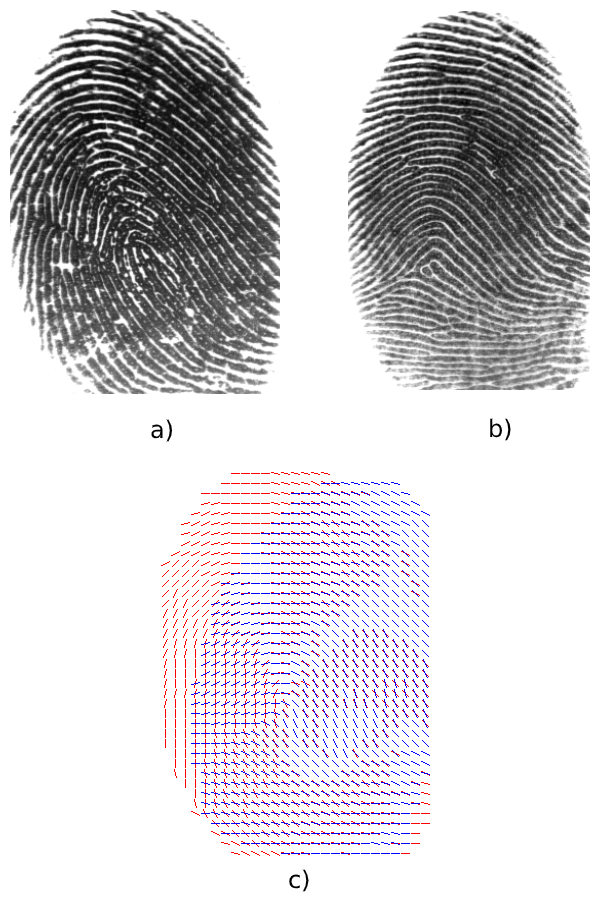
\includegraphics[width=0.8\linewidth]{images/prunik.png}}\\
            \caption{a)otisk 1 b) otisk 2 c) výsledek průniku orientovaných polí}
            \label{fig:prunik}
    \end{figure}
    \subsection{Stanovení frekvenční charakteristiky otisku}
    Úrovně šedé v okolí linií mohou být modelovány jako sinusovka, pro případy kde se nevyskytuje v lokálním okolí minutiae nebo singulární bod. Pro tyto případy je lokální frekvence další důležitou složkou obrazu otisku prstu. Mějme $\mathcal{G}$ značící normalizovaný obraz otisku a $\mathcal{O}$ orientované pole vypočítané jako je popsáno v minulé sekci. Poté:
    \begin{enumerate}
        \item Rozdělíme si $\mathcal{G}$ na w x w bloky, kde w = w z prvního kroku orientovaného pole.
        \item  Pro každý blok s prostředkem v (i,j), spočítáme pole l $x$ w, otočené o úhel $\mathcal{O}(i,j)$.:
              \begin{equation}
                X[k]=\frac{1}{w} \sum_{d=0}^{w-1} \mathcal{G}(u, v), \quad k=0,1, \ldots, l-1
             \end{equation}
             \begin{equation}
                \begin{multlined}
                    u=i+\left(d-\frac{w}{2}\right) \cos \mathcal{O}(i, j)+\\
                    \left(k-\frac{l}{2}\right) \sin \mathcal{O}(i, j)
                \end{multlined}
             \end{equation}
             
             \begin{equation}
                \begin{multlined}
                    v=j+\left(d-\frac{w}{2}\right) \sin \mathcal{O}(i, j)+\\ 
                    \left(k-\frac{l}{2}\right) \cos \mathcal{O}(i, j)
                \end{multlined}
             \end{equation}
        \item Pokud se žádné singulární ani minutiae body neobjeví v orientovaném poli, x-signture formuje sinusový tvar vlny. Nechť $\mathcal{T}(i,j)$ je průměrný počet pixelů mezi dvěma vrcholy. Poté je frekvence stanovena jako:
        \begin{equation}
            \Omega(i, j)=1 / \mathcal{T}(i, j)
         \end{equation}
    \end{enumerate}\cite{ori}
    
    Příklad výsledku je vidět na obrázku \ref{fig:freq}.
    \begin{figure}[H]
        \centering
            {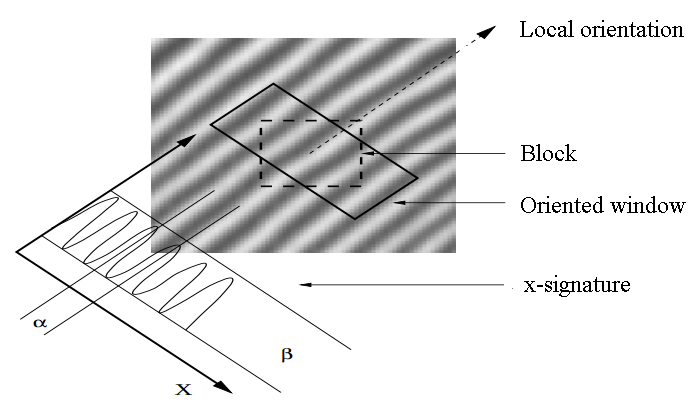
\includegraphics[width=0.4\linewidth]{images/freq.png}}\\
            \caption{Frekvenční charakteristika otisku z obrázku \ref{fig:ori}}
            \label{fig:freq}
    \end{figure}
    \subsection{Minutiae}\label{miniatue}
        Linie a údolí se na otisku prstu střídají a proudí jednotným směrem. Federal Bureau of Investigation roku 1984 našel 18 vlastností charakterizujících otisk prstu. Aktuálně známe přes 150 různých lokálních vlastností linií. Tyto lokální vlastnosti nejsou rovnoměrně rozloženy. Detekce většiny z nich převážně záleží na kvalitě snímku otisku a jsou málokdy viděny. Dvě vlastnosti s největším výskytem jsou zakončení linie a rozdvojení linie, viz. obrázek \ref{fig:mini_1} \cite{mini_1}. Hromadně se tyto vlastnosti nazývají minutiae. Většina aplikací pro extrakci a porovnání minutiae používají právě dvě uvedené vlastnosti. Na otisku prstu zaznamenaném v dobré kvalitě může být nalezeno okolo 40 až 100 minutiae.
        
        \begin{figure}[H]
            \centering
                {\includegraphics[width=0.8\linewidth]{images/mini_1.jpg}}\\
                \caption{a) zakončení linie, b) rozdvojení linie \cite{mini_1}}
                \label{fig:mini_1}
        \end{figure}
        
        Další typy minutiea jsou kombinací dvou uvedených. Každé zakončení linie a rozdvojení linie se skládá ze tří vlastností a to (x,y) souřadnice, kde se nachází s lokální orientace $\theta$. Tato reprezentace otisků prstů je používána z důvodu zmenšení dat v databázi, ale také bezpečnosti, kdy sestrojit otisk prstu ze získaných minutiae je prakticky nemožné.
        
        V projektu je použit algoritmus pracující na extrakci minutiae pomocí thinningu. Pro extrakci minutiae je zapotřebí prvně spočítat orientované pole popsané výše. Následně rozlišit pozadí a otisk. Důležitým krokem je extrakce linií, neboli vytvořit černobílí obrázek, kde linie jsou tvořeny černou barvou a údolí s pozadím bílou. Posledním krokem extrakce linií je thinning, kde je extrakce převedena na binární matici, kde linie jsou tvořeny čárami o šířce jeden pixel s hodnotou 1 a pozadí má hodnotu 0. Dosažení thinningu je pomocí použití morfologických operací skeletonizace a vzdálenostní tranformace na inverzní výsledek extrakce linií. Následně je výsledek thinningu očištěn od osamocených pixelů. Výsleden thinningu může být vidět v obrázku \ref{fig:thinning}.
        
        \begin{figure}[H]
            \centering
                {\includegraphics[width=0.4\linewidth]{images/thinned.png}}\\
                \caption{Výsledek operace thinningu otisku z obrázku \ref{fig:ori}}
                \label{fig:thinning}
        \end{figure}
        
        Následná extrakce minutiae je provedena pomocí použití metody "crossing number" na okolí bodu P ve vzdálenosti 1. Neboli na jeho 8 okolních pixelů:
        \begin{equation}
            C N=0.5 \sum_{i=1}^{8}\left|P_{i}-P_{i+1}\right|, \quad P_{9}=P_{1}
        \end{equation}
        Následně dojde v postprocessingu k odstranění falešných minutiae. První částí je ridge counting. Pomocí ridge counting se určí, kolik linií prochází nebo se dotýká přímky, která je spojnicí mezi jádrem a deltou. Pro tuto operaci je zapotřebí co nejpřesněji určit deltu a jádro otisku. Následně:
        \begin{itemize}
            \item Pokud přímka prochází místem rozdvojení linie, poté jsou dvě linie započítány.
            \item Pokud se přímka dotýká ostrovu (místo mezi dvěmi rozdvojeními), nebo tečky, poté je započítána jedna linie
            \item Údolí musí být přerušeno linií mezi deltou a jádrem, jinak je jedna linie odečtena. (Vztahuje se pouze na linie ve tvaru smyčky.
        \end{itemize}
        
        Následně je vypočítán průměr počtu pixelů mezi dvěma přilehlými liniemi. Neboli je podělen výsledek ridge counting vzdáleností mezi jádrem otisku a deltou. Vzdálenost mezi dvěma minutiae musí být poté větší než tato průměrná hodnota. Algoritmus použitý v projektu pro extrakci minutiae je implementován dle paperu \cite{thinning}.
        
        \subsubsection{Jádro a Delta}
        V použitém algoritmu je ještě zapotřebí popsat jádro otisku a deltu. Jedná se o skupinu high-level vlastností, tzv. singulární body. Otisk prstu může mít žádné nebo více jader. Jádro se vyskytuje u středu otisku prstu a je tvořeno ze "závitu" - whorl , kdy jako jádro je detekován střed závitu, nebo ze "smyčky" - loop, kdy jako core je detekován nejvyšší bod nejnižší smyčky. Delta je poté tvořena liniemi ve směru trojúhelníku, které z ní vyzařují. Delta a jádro jsou vidět na obrázku \ref{fig:core}.
        \begin{figure}[H]
            \centering
                {\includegraphics[width=0.5\linewidth]{images/core.jpg}}\\
                \caption{Ukázka detekované delty a jádra (core) \cite{core}}
                \label{fig:core}
        \end{figure}
        
        Pro detekci jádra v otisku byl použit algoritmus založený na metodě Poincaré Index \cite{pointcare}, který na základě okolí ve vzdálenosti 1 (8 okolních pixelů) zjistí, zda se jedná o delta / jádro / nic.
        
\section{Cutline}
    Jedná se o přímku okolo které se vyskytuje nejvíce minutiae a při generování nového otisku zajišťuje, že v otisku bude dostatečné množství minutiae z obou otisků. Přímka se počítá po provedení všech dříve popsaných operacích tedy na zarovnaných a oříznutých otiscích od částí neprůniku i s jejich orientovanými poli. Minutiae extrahované z těchto otisků označíme jako $T^1$ pro otisk 1. a $T^2$ pro otisk 2.
    
    Následně označíme $\rho = (\rho_x, \rho_y)$ jako barycentrum. Ve článku není uvedeno, o co se přesně jedná, tak jsem použil jádro / deltu otisku, přičemž pokud vypadne při průniku je za barycentrum označen střed otisku.
    
    Poté má přímka $l$ (cutline) parametry:
    \begin{equation}
        \begin{array}{l}
        a_{l} \cdot x+b_{l} \cdot y+c_{l}=0 \\
        a_{l}=\sin (\beta), \quad b_{l}=\cos (\beta) \\
        c_{l}=-\rho_{x} \cdot \sin (\beta)-\rho_{y} \cdot \cos (\beta)
        \end{array}
    \end{equation}
    Nyní je přímka točena okolo barycentra předurčeným krokem v rozsahu $(0^{\circ},180^{\circ})$. Pro každý úhel $\beta$ je určeno skóre přímky:
    \begin{equation}
        S_{c}=\omega_{o} \cdot S_{o}+\omega_{v} \cdot S_{v}+\omega_{m} \cdot S_{m}
    \end{equation}
    Kde $S_o$ je podobnost orientovaných polí, $S_v$ je podobnost frekvenčních charakteristik, $S_m$ je skóre, které slouží k ohodnocení vzhledem k generování otisku podobnému oběma na základě nalezených minutiae otisku 1: $T_1$, a otisku 2: $T_2$. $\omega_{o}, \omega_{v}, \omega_{m}$ jsou poté váhy jednotlivých složek v rozsahu \\$<0;1>$, $\omega_{o} + \omega_{v} + \omega_{m} = 1$.
    \begin{equation}
        S_{o}=\frac{\sum_{(i, j) \in C}\left(r_{i, j}^{1}+r_{i, j}^{2}\right) \cdot \psi\left(\theta_{i, j}^{1}, \theta_{i, j}^{2}\right)}{\sum_{(i, j) \in C}\left(r_{i, j}^{1}+r_{i, j}^{2}\right)}
    \end{equation}
    \begin{equation}
        S_{v}=\frac{\sum_{(i, j) \in C}\left(1-\frac{\left|v_{i, j}^{1}-v_{i, j}^{2}\right|}{\left(\max _{F}-\min _{F}\right)}\right)}{|C|}
    \end{equation}
    C obsahuje pouze prvky, které jsou od cutline $l$ vzdáleny maximálně $d_{max}$ a jsou průnikem orientovaných polí $\hat{O}^{1}, \hat{O}^{2}$ tedy :
    \begin{equation}
      \begin{multlined}
          C=\{(i, j) |(i, j) \in\left(V_{\hat{O}^{1}} \cap V_{\hat{O}^{2}}\right) \wedge \\\operatorname{dist}_{l}(i, j) \leq d_{\max }\}
      \end{multlined}
     \end{equation}
     \begin{equation}
         \operatorname{dist}_{l}(x, y)=\frac{\left|a_{l} \cdot x+b_{l} \cdot y+c_{l}\right|}{\sqrt{a_{l}^{2}+b_{l}^{2}}}
     \end{equation}
     \begin{equation}
         S_{m}=\max \left(\zeta_{m}\left(T^{1}, T^{2}\right), \zeta_{m}\left(T^{2}, T^{1}\right)\right)
     \end{equation}
     \begin{equation}
     \begin{multlined}
         \zeta_{m}(A, B)=\\\frac{Z\left(|A|_{l}^{P}, \mu_{m}, \tau_{m}\right)+Z\left(|B|_{l}^{N}, \mu_{m}, \tau_{m}\right)}{2}
     \end{multlined}
     \end{equation}
     kde $|T|_{l}^{P}$ a $|T|_{l}^{N}$ označují minutiae, které spadají nad přímku a pod $l$. Neboli:
     \begin{equation}
         \begin{array}{l}
            |T|_{l}^{P}=\left|\left\{m \in T | \phi_{l}\left(m_{x}, m_{y}\right) \geq 0\right\}\right| \\
            |T|_{l}^{N}=\left|\left\{m \in T | \phi_{l}\left(m_{x}, m_{y}\right)<0\right\}\right|
        \end{array}
     \end{equation}
     
     Z je sigmoidní funkce kontrolována parametry $\mu$ a $\tau$, které zajistí, že výsledek bude vždy mezi 0 a 1:
     \begin{equation}
         Z(v, \mu, \tau)=\frac{1}{1+e^{-\tau(v-\mu)}}
     \end{equation}
     Jako cutline je označena cutline s nejvyšší hodnotou skóre $S_c$.\cite{main}
     Příklad cutline je vidět na \\ obrázku \ref{fig:cutline}.
     \begin{figure}[H]
        \centering
            {\includegraphics[width=0.8\linewidth]{images/cut.png}}\\
            \caption{a) cutline na otisku 1 b) cutline na otisku 2}
            \label{fig:cutline}
    \end{figure}
\section{Generování otisku dvojí identity}
    Zvolil jsem metodu generování otisku na základě obrazu. Otisk je generován pomocí sloučení průniků otisků. Nechť $\hat{F}^{p}$ je část otisků nad cutline a $\hat{F}^{n}$ je část otisků pod cutline, které určíme následovně:
    \begin{equation}
        (p, n)=\left\{\begin{array}{ll}
(1,2) & \text { if } \zeta_{m}\left(T^{1}, T^{2}\right) \geq \zeta_{m}\left(T^{2}, T^{1}\right) \\
(2,1) & \text { otherwise }
\end{array}\right.
    \end{equation}
    
    Poté je otisk generován následovně: 
    \begin{equation}
        D^{I}(x, y)=w_{x, y}^{l_{\max }} \cdot \hat{F}^{p}(x, y)+\left(1-w_{x, y}^{l_{m a x}}\right) \cdot \hat{F}^{n}(x, y)
    \end{equation}
    kde $w_{x, y}^{l_{\max }}$ je váha pro vyvážení smíchání otisků v blízkosti cutline.
    
    \begin{equation}
        w_{x, y}^{l_{\max }}=\left\{\begin{array}{c}
1-\max \left(0, \frac{d_{\max }-\operatorname{dist}_{\max }(x, y)}{2 \cdot d_{\max }}\right) \\
\operatorname{pokud} a_{\ln a x} \cdot x+b_{\ln a x} \cdot y+c_{\ln a x} \geq 0 \\
\max \left(0, \frac{d_{\max }-\operatorname{dist}_{\ln a_{a x}}(x, y)}{2 \cdot d_{\max }}\right) \text { jinak }
\end{array}\right.
    \end{equation}
    Výsledek takovéto operace je vidět na obrázku \ref{fig:morph}.
     \begin{figure}[H]
        \centering
            {\includegraphics[width=0.5\linewidth]{images/morph_res.png}}\\
            \caption{Výsledek morphingu otisků z obrázku \ref{fig:prunik}}
            \label{fig:morph}
    \end{figure}
\section{Implementace}
    Aplikace je převážně založena na článku \cite{main} a je implementována v jazyce Python verze 3.7.5. Dále byly použity knihovny Numpy pro práci s maticemi, SciPy a OpenCV pro práci s obrazem. Pro thining a minutiae byla použita knihovna z git repozitáře \cite{gitlib}.

\section{Dataset}
    Dataset byl použit pro zkušební generování otisků prstů zde popsanou metodou. Bylo využito malé databáze s obsahem 80 otisků prstů Set "B" of Database 1 z \cite{database}.


\bibliographystyle{plain}
\renewcommand{\refname}{Použitá literatura}
\bibliography{bibliography.bib}
\end{multicols*}
\end{document}
